\documentclass[10pt]{article}
\usepackage[utf8]{inputenc}
\usepackage[papersize={17in, 11in}]{geometry}
\usepackage[absolute]{textpos}
\usepackage{graphicx}
\TPGrid[1.0in, 1.0in]{23}{24}
\usepackage{palatino}
\parindent=0pt
\parskip=12pt
\usepackage{nopageno}
\begin{document}

\begin{textblock}{23} (0, 1)
\center\huge INSTRUMENTATION
\end{textblock}

\begin{textblock}{9} (7, 3)

    \begin{itemize}

        \item[-] \textbf{Flute}, with brazil nut shaker \\

        \item[-] \textbf{Oboe} \\

        \item[-] \textbf{Clarinet in b-flat}, with brazil nut shaker \\

        \item[-] \textbf{Percussion} \\

            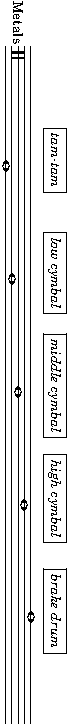
\includegraphics{preface-percussion-metals.pdf} \\ \\ \\
            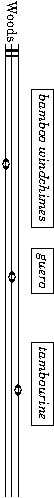
\includegraphics{preface-percussion-woods.pdf} \\ \\ \\
            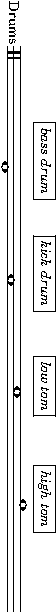
\includegraphics{preface-percussion-drums.pdf} \\

            Mallets: hard sticks or bare hands, wire brushes, superballs \\

        \item[-] \textbf{Piano} \\

            Prepare the lowest and highest octaves with any combination of
            felt, tape or rubber to dampen and distort the timbre of the
            strings. \\

            Guero passages should be played with a piece of hard paper or
            plastic, on the keys. The register of the motions is left to the
            performer. \\

        \item[-] \textbf{Violin}, with brazil nut shaker \\

        \item[-] \textbf{Viola}, with brazil nut shaker \\

        \item[-] \textbf{Cello}

    \end{itemize}

\end{textblock}


\end{document}